If we have an SPL with certain requirements that must hold for every product then we want to apply verification techniques to formally verify that indeed every product satisfies the requirements. We could verify every product individually, however verification is expensive in terms of computing time and the number of different products can grow large. Differences in behaviour between products might be very small; large parts of the different products might behave similar. In this thesis we aim to exploit commonalities between products to find a method that verifies an SPL in a more efficient way than verifying every product independently.

First we take a look at a method of modelling the behaviour of the different products in an SPL, namely \textit{featured transition systems} (FTSs). An FTS extends the definition an LTS to express variability, it does so by introducing \textit{features} and \textit{products}. Features are options that can be enabled or disabled for the system. A product is a feature assignments, i.e. a set of features that is enabled for that product. Not all products are valid; some features might be mutually exclusive for example. To express the relation between features one can use feature diagrams as explained in \cite{Classen2013FeaturedTS}. Feature diagrams offer a nice way of expressing which feature assignments are valid, however for simplicity we represent the collection of valid products simply as a set of feature assignments. 

An FTS models the behaviour of multiple products by guarding transitions with boolean expressions over the features such that the transition is only enabled for products that satisfy the guard.

Let $\mathbb{B}(A)$ denote the set of all boolean expressions over the set of boolean variables $A$, a boolean expression is a function that maps a boolean assignment to either true of false. A boolean expression over a set of features is called a feature expression, it maps a feature assignment, i.e. a product, to either true or false. Given boolean expression $f$ and boolean variable assignment $p$ we write $p \models f$ if and only if $f$ is true for $p$ and write $p \not\models f$ otherwise. Boolean expression $\top$ denotes the boolean expression that is satisfied by all boolean assignments.
\begin{definition}[\cite{Classen2013FeaturedTS}]
	\label{def_fts} A featured transition system (FTS) is a tuple $M = (S, Act, trans, s_0, N, P, \gamma)$, where:
	\begin{itemize}
		\item $S, Act, trans, s_0$ are defined as in an LTS,
		\item $N$ is a non-empty set of features,
		\item $P \subseteq 2^N$ is a non-empty set of products, i.e. feature assignments, that are valid,
		\item $\gamma : trans \rightarrow \mathbb{B}(N)$ is a total function, labelling each transition with a feature expression.
	\end{itemize}
\end{definition}
A transition $s \xrightarrow a s'$ and $\gamma(s,a,s') = f$ is denoted by $s \xrightarrow {a\ |\ f} s'$. FTSs are presented similarly as LTSs, the labels of the transition are expanded to represent both the action and the feature expression associated with it.

\begin{example}[\cite{FamBasedModelCheckingWithMCRL2}]
	Consider a coffee machine that has two variants: in the first variant it takes a single coin and serves a standard coffee, in the second variant the machine either serves a standard coffee after a coin is inserted or it takes another coin after which it serves an xxl coffee. Note that there is no variant that only serves xxl coffees. We introduce two features: $\$$ which, if enabled, allows the coffee machine to serve xxl coffees and $\officialeuro$ which, if enabled, allows the coffee machine to serve standard coffees. The valid products are: $\{\{\officialeuro\},\{\officialeuro,\$\}\}$. This FTS is depicted in Figure \ref{fig:coffeemachinefts}.
	
	\begin{figure}[h]
		\centering
		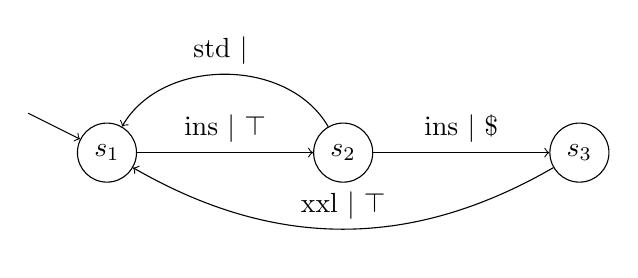
\begin{tikzpicture}[->]
			\tikzstyle{state} = [circle,draw,minimum size=0.75cm]
			
			\node[state] (s1) at (1,1.5) {$s_1$};
			\node[state] (s2) at (4,1.5) {$s_2$};
			\node[state] (s3) at (7,1.5) {$s_3$};
			
			\path (s1) edge node[above]{ins $|\ \top$} (s2) ;
			\path (s2) edge[bend right=60] node[above]{std $|\ \officialeuro$} (s1) ;
			\path (s2) edge node [above]{ins $|\ \$$} (s3);
			\path (s3) edge[bend left] node [above]{xxl $|\ \top$} (s1);
			\path (0,2) edge (s1);
		\end{tikzpicture}
		\caption[Coffee machine LTS]{Coffee machine FTS $C$}
		\label{fig:coffeemachinefts}
	\end{figure}
	
\end{example}
An FTS expresses the behaviour of multiple products. The behaviour of a single product can be derived by simply removing all the transitions from the FTS for which the product does not satisfy the feature expression guarding the transition. We call this a \textit{projection}.

\begin{definition}[\cite{Classen2013FeaturedTS}]
	\label{def_fts_proj}
	The projection of FTS $M = (S, Act, trans, s_0, N, P, \gamma)$ onto product $p \in P$, denoted by $M_{|p}$, is the LTS $(S,Act,trans', s_0)$, where $trans' = \{t \in trans\ |\ p \models \gamma(t)\}$.
\end{definition}

\begin{example}[\cite{FamBasedModelCheckingWithMCRL2}]
	The coffee machine example can be projected to its two products, which results in the LTSs in Figure \ref{fig:cofeemachineftsproj}.
	\begin{figure}[h]
		\centering
		\begin{subfigure}{.5\textwidth}
			\centering
			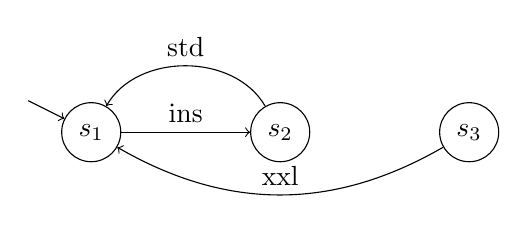
\begin{tikzpicture}[->,scale=0.8]
				\tikzstyle{state} = [circle,draw,minimum size=0.75cm]
				
				\node[state] (s1) at (1,1.5) {$s_1$};
				\node[state] (s2) at (4,1.5) {$s_2$};
				\node[state] (s3) at (7,1.5) {$s_3$};
				
				\path (s1) edge node[above]{ins} (s2) ;
				\path (s2) edge[bend right=60] node[above]{std} (s1) ;
				\path (s3) edge[bend left] node [above]{xxl} (s1);
				\path (0,2) edge (s1);
			\end{tikzpicture}\
			\caption[$C_{|\{\$\}}$]{$C$ projected to the \textit{euro} product: $C_{|\{\officialeuro\}}$}
			\label{fig:coffeemachineftsprojeuro}
		\end{subfigure}%
		\begin{subfigure}{.5\textwidth}
			\centering
			
			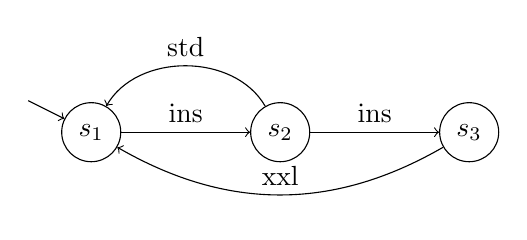
\begin{tikzpicture}[->,scale=0.8]
				\tikzstyle{state} = [circle,draw,minimum size=0.75cm]
				
				\node[state] (s1) at (1,1.5) {$s_1$};
				\node[state] (s2) at (4,1.5) {$s_2$};
				\node[state] (s3) at (7,1.5) {$s_3$};
				
				\path (s1) edge node[above]{ins} (s2) ;
				\path (s2) edge[bend right=60] node[above]{std} (s1) ;
				\path (s2) edge node [above]{ins} (s3);
				\path (s3) edge[bend left] node [above]{xxl} (s1);
				\path (0,2) edge (s1);
			\end{tikzpicture}\
			\caption[$C_{|\{\$\}}$]{$C$ projected to the \textit{euro and dollar} product: $C_{|\{\officialeuro,\$\}}$}
			\label{fig:coffeemachineftsprojdollar}
		\end{subfigure}%
		\caption{Projections of the coffee machine FTS}
		\label{fig:cofeemachineftsproj}
	\end{figure}
\end{example}

\paragraph{Problem statement}
Given an FTS $M$, that models the behaviour of an SPL, with products $P$ and modal $\mu$-calculus formula $\varphi$ we want to verify that $\varphi$ holds for every product in $P$. Formally we want to find set $P_s$ such that:
\begin{itemize}
	\item for every $p \in P_s$ we have $M_{|p} \models \varphi$ and
	\item for every $p \in P \backslash P_s$ we have $M_{|p} \not\models \varphi$.
\end{itemize}
We aim to find $P_s$ in a way that utilizes the commonalities in behaviour between the different products.